\chapter{Motivation}

What is ``probability''? What is ``statistics''? Why are they
important?

This introductory chapter is a gentle introduction to these concepts,
in later chapters we will go deeper and provide you with specific
tools for solving specific problems.

This chapter provides a high level panorama for the rest of the
book. Its goal is to demonstrate why probability and statistics are so
important to a computer scientist. Hopefully, this chapter will make
you think about some interesting questions.

However, this chapter will not provide answers. Your grade will
probably not be impacted by whether or not you read it. However,
motivation is important, and makes your learning experience more
enjoyable, so I hope you will read this chapter!

\section{AB tests of online ads}

Suppose you own a web site and that you make money by placing
advertisements on the pages of your site. The way advertisers pay the web
site is based on ``click through'' events (CT)\footnote{Actually, CTs are
  only part of the payment contract, there are many other factors that effect
  the payment. For simplicity we concentrate here on CTs.} 
A CT is the event that a particular ad is displayed on a
web page (also called an {\em impression}) and the user clicks on the
ad to go to the advertiser's site. That click is an indication of some
interest on the part of the visitor. You, the website owner, get
paid whenever a CT occurs.

For simplicity, let's consider a single static page, with a single
location on the page for presenting the advertisement and just two
alternative ads to place in this location, which we will call ad A and
ad B. 

How can we figure out which is the best advertisement to put on the
page?

One thing we can do is this: each time the web page is presented,
choose one of the possible ads in an alternating manner
(B,A,B,A,B,... ) and present the page to the visitor. We then see if
the visitor clicks on the advertisement, producing a CT. Suppose that
the number of visitors to the page is very large. The {\em law of
  large numbers} tells us that the fraction of CTs among all the
impressions of A (or B) converges to a particular limit.  This number
is called the ``click through rate'' or CTR for the ad. If the
paymnent for all ads are equal then the ad with the highest CTR is the
best one to place on the page.

The law of large numbers is a fundamental law of probability and
statistics, we will come back to it later.

\iffalse
This is an example of {\em Statistical inference}. Statistical
inference is a set of methods for analyzing collected data and drawing
conclusions about the real world from that data. 
\fi

A single page-visit, together with a flag indicating whether or not
the ad was clicked is called an {\em observation} or an {\em outcome}
and the sequence of $n$ independent observations is called a {\em
  sample}. Statistics is a set of methods for drawing conclusions from
random samples. The process that is generating the observations is
called a {\em Stochastic Process}. The conclusions we draw are stated
as properties of this stochastic process. In our case, we conclude
that one ad has a higher CTR than the other.

Suppose first we have 10,000 impressions for each of the two ads, and
suppose we got 200 CTs for ad A and 150 CTs for ad B. All other things
being equal, we can conclude the the CTR for ad A is about \%$2$ and for
ad B is about \%$1.5$ and our preference should be to present
ad A rather than ad B. However, it is intuitively clear that this
conclusion is not a very confident one, as it rests on a difference of
$50$ in the number of CTs.

As we cannot make a confident conclusions, we continue placing the ads
in an alternating order (A,B,A,B,...) until we have 1,000,000
impressions of each type. Suppose at that point that we have 200,000
CTs for A and 150,000 CT's for B. The CTR's are the same as before:
\%$2$ for A and  \%$1.5$  for B. Again, we conclude that A is a
better ad than B. In this case the difference in
the number of CTs is 50,000 rather than 50 and our intuition tells us
that we can be confident that A is the ad with the higher CTR.

How can we justify this intuition?

To explain and quantify this intuition we use probability theory.

\section{Probability Theory}

Probability theory is a branch of mathematics which is the foundation
for statistics. This is similar to the way in which discrete math and
the theory of computation are the foundation for writing correct and
efficient computer programs.

The input for statistical inference is data collected from the real
world, and the output is a {\em model} of the real world. Probability
theory works in the opposite direction. The input is a {\em stochastic
  process} or a {\em model}, and the outputs are probabilities of {\em
  events}.

Specifically, in our case, we can model the process generating the
click-through observation using two biased coins. An {\em unbiased
  coin} is a symmetric coin for which the probability of landing
``heads'' is equal to the probability of landing ``tails''.  A {\em
  biased} coin is one where these probabilities are different.  In our
case the coin for ad A has probability $P_A$ of landing ``heads''
which is equal to the probability that a random visitor will click on
the ad. Similarly $P_B$ corresponds to the probability that the coin B
lands ``heads'' which is equal to the probability that a random
visitor will click on the ad B. More succinctly, $P_A$ is the CTR of
ad A and $P_B$ is the CTR of ad B.

The question that we want to answer is which probability is larger, is
$P_A>P_B$ or is the reverse true: $P_A \leq P_B$ ?

Suppose we are are in the first case in which we presented each
advertisement $10,000$ times and got $200$ click-throughs for ad A and
$150$ for ad B. Clearly, it seems that $P_A>P_B$. But how {\em
  confident} can we be that this is indeed the case?

To answer this question we consider two alternative {\em statistical
hypotheses}: the first is that $P_A>P_B$, the second is that $P_A
\leq P_B$. 

We then find the two settings of $P_A$ and $P_B$ that conform with
each hypothesis and give the highest probability for the data.  For
the hypothesis $P_A>P_B$ we get the highest probability when
$P_A=0.02,P_B=0.015$. For the alternative hypothesis we use
$P_A=0.0175,P_B=0.0175$, i.e. we place the two probabilities midway
between the two observed rates.\footnote{Strictly speaking the
  mid-point is not the highest probability setting, but the difference
  is small and we ignore it here.}.

We now compute the probability of the observed data corresponding to
each of these two settings, which correspond to the two alternative
hypotheses. Clearly the probability of the data under the first
settings will be higher than the probability of the second, so if we
take the ratio of the two probabilities we expect to get a number
smaller than 1. The question is, how much smaller than 1?

Computing this ratio is not a trivial matter. You will learn how to
do it later in the course. For now, I'll tell you that when the number
of impressions for each ad is 10,000 the ratio is $0.6766$, while when
the number of impressions is 1,000,000 the ratio is smaller than
$10^{-16} = 1/10,000,000,000,000,000$. In other words, in the first
case we cannot conclude which ad is better with any degree of
confidence, while in the second case we can be pretty sure that the
first ad is better.

Note how dramatic is the improvement in confidence: increasing the
sample size from 10,000 to 1,000,000 transforms a relative gap of 0.5\%
from an insignificant gap to one from which can conclude something
almost surely. Keep this very small number $10^{-16}$ in mind, we will
get back to it later in the course.

\section{Low probability vs. certainty}
In computer science we are used to giving absolute guarantees: we
expect that hardware and software will give the correct answer each 
and every time. The whole concept of ``debugging'' a program is based
on the assumption that every mistake can be traced back to a
particular part of the computer code and thereby eliminated. 

However, in the real world, many computer errors cannot be
reconstructed, explained, or corrected. The more realistic goal is
becoming to have computer systems that minimize the number of errors
without necessarily correcting all of the bugs.

Certainty is golden; however, in the real world, having a guarantee
that some error will occur no more than once every $10^{16}$ attempts
is a very strong guarantee. Increasing $n$ from $1,000,000$ to
$100,000,000$ will reduce the probability to 1 in $10^{64}$.

\section{Average and Mean}
The number of observations, or the size of the sample $n$ is of
central importance in probability and in statistics. In general, as
$n$ increases we reach the ``law of large numbers'' which tells us
that averages converge to the means.

People sometimes use ``mean'' and ``average'' interchangeably. However
in probability and statistics the difference is very important. Going back to the
click-through example above. consider the sequence of presentations of
the ad A, each resulting either in a click (1) or in a non-click
(0). For example, suppose the sequence is:
\[
0,0,0,1,0,0,0,0,1,1,0,0,0,0,0,0,0,1,0,0,0,0,0,0,...
\] 
The {\em average} of the first 5 outcomes is $1/5$. If we compute
the average of the first $n$ outcome for $n=1,2,3,...$ we get a
sequence of {\em running averages}:
\[
0,0,0,1/3,1/4,1/5,1/6,1/7,2/8,3/9,3/10,3/11,...
\]
As the sequence of outcomes is random, the sequence of averages is
also random. By this we mean that if we collected a difference
sequence of observations from the same source, we are very likely to
get a different sequence. In the language of probability, we say that
the outcomes and the averages are {\em random variables}.

The terms: ``empirical'', ``observational'', ``sample'', ``random
variable'' indicate that the quantity we are referring to is likely to
change if we repeat the same experiment.

The mean, on the other hand, is {\em not} a random variable. The mean
is a {\em constant property of the source}, in this case, the mean is
equal to $P_A,P_B$ which are the CTRs for ad A and ad B
respectively. In fact $P_A$ and $P_B$ are the quantities that
determine which ad is more profitable.\footnote{Other terms that are
  used to refer to the average are the {\em empirical mean} or the
  {\em sample mean}. These can be easily confused with the regular
  mean. However, they are random variables, not constants.}

The law of large numbers connects the sequence of running averages and
the mean. What the law of large number says (roughly) is that the
sequence of averages converges to the mean. In other words, if $n$ is
large enough, the difference between the average and the mean is going
to be small with high probability.

\section{Monte Carlo Simulations}
As I said above, computing the probability flipping a biased coin $n$
times will result in $k$ heads and $n-k$ tails is not
trivial and requires some knowledge of probability theory. However,
symbolic derivation (also called ``closed form solution'') is not the
only way to arrive at the answer. There is another way which is called
``monte-carlo simulations''.

A monte-carlo simulation is a computer program that simulates the
process of generating the outcomes. It uses ``pseudo-random number
generators'' about which we will learn later on. For now it suffices
to describe the pseudo-random number generator as a function {\tt
  random(p)}. Every time {\tt random(p)} is called it returns a bit
whose value is $1$ with probability $p$ and $0$ with probability
$1-p$.

\begin{figure}[p]
\begin{center}
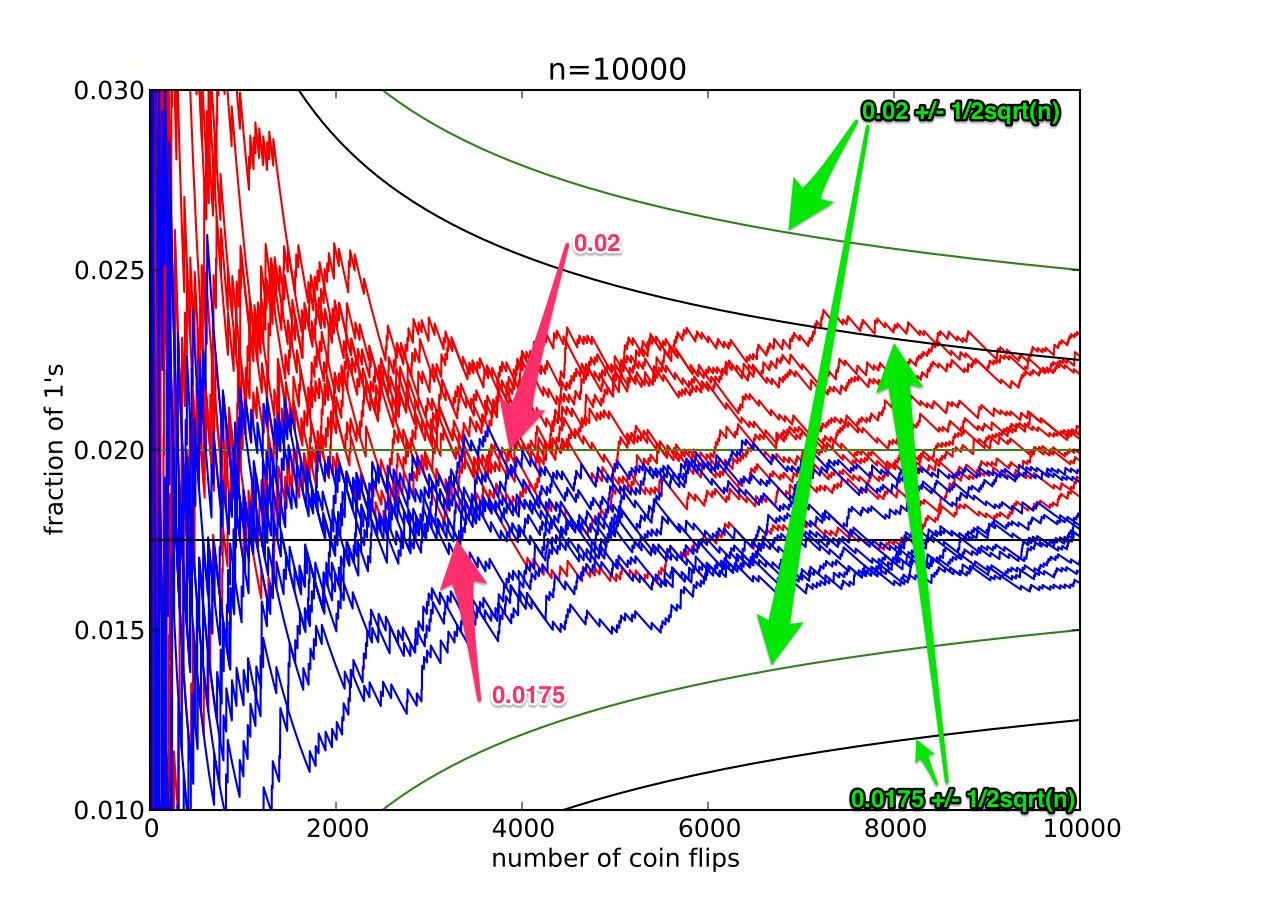
\includegraphics[width=5in]{figs/averages10000.png}
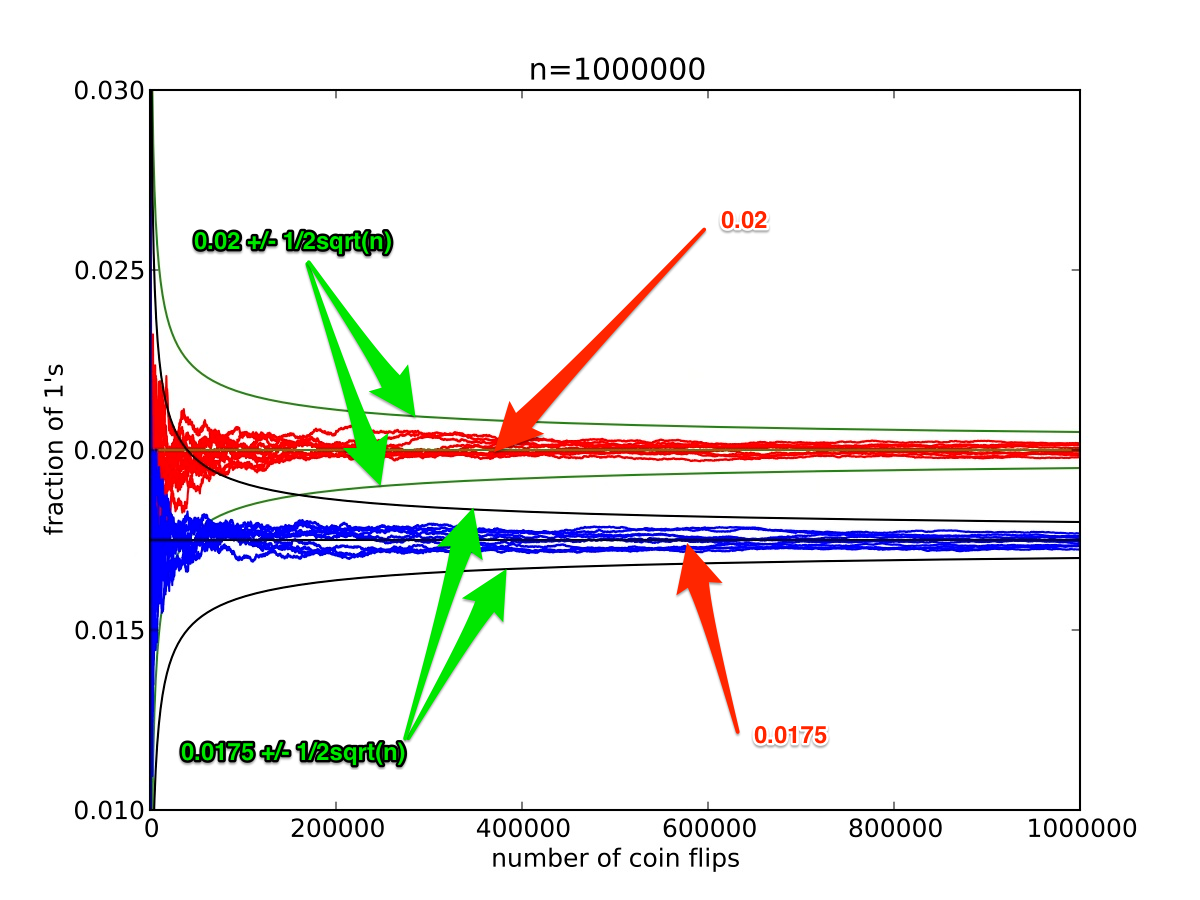
\includegraphics[width=5in]{figs/averages1000000.png}
\end{center}
\caption{\label{fig:Averages} Trajectories of running averages of
  random sequences generated by a biased coin with sides that say
  ``0'' and ``1''. There are two sets of 10 trajectories. The red
  trajectories correspond to sequences of random coin flips where the
  probability of 1 is $0.02$. The blue trajectories correspond to
  sequences of random coin flips where the probability of a 1 is
  $0.0175$}
\end{figure}

Using a random number generator we can create samples of the type
described above, compute running averages of these sample, and plot
them, see Figure~\ref{fig:Averages}.\footnote{The code is available
  via GitHub: {\tt
    https://github.com/yoavfreund/CSE103-code/blob/master/MonteCarlo/monteCarlo.py}}
These plots demostrate why there is such a qualitative difference
between a sample of size $10,000$ and a sample of size
$1,000,000$. The red trajectories correspond to sequences generated by
a coin with bias $P=0.02$ while the blue trajectories were generated
by a coin with bias $P=0.0175$ (the most likely value for $P_A$ which
allows for $P_A \leq P_B$). Looking at the bottom figure,
corresponding to $n=1,000,000$ we see that the sequences all converge
to their mean, as is predicted by the law of large numbers. However,
if we look at the top figure, where $n=10,000$, we see that the red
trajectories and the blue trajectories are not well separated. The red
and the blue lines cross each other many times.

What does this mean for drawing conclusions about whether $P_A>P_B$ ?
The one experiment that we did corresponds to two sequences of length
$10,000$, one for each ad. In this figure we are focusing on the
sequence for ad A. We know that this sequence ended up at $k=200$ when
$n=10,000$. We want to compare the probability that this sequence was
generated by a coin with bias $P_A=0.02$ to the probability that it
was generated by a coin with bias $P_A=0.0175$. What we see from the
sample is that the probabilities are comparable. It is hard to say
what is the ratio of the probabilities, but if instead of generating
10 trajectories we generated 10,000 trajectories we could probably
give an accurate estimate of the ratio.

Compare that situation to the one when $n=1,000,000$ and you see that
now the separation between the two sets of trajectories is perfect. This
means that the probability of a blue trajectory having $k=20,000$ is
miniscule.

These graphs give us a useful intuition for the behaviour of running
averages of coin flips. We can clearly see the effect of the law of
large numbers.

What's more, probability theory tells us that the rate at which the
running averages converge to the mean is $O(1/\sqrt{n})$. We
demonstrate this in the figures by drawing around the horizontal line
representing the means the envelope which represents the rate at which
a random sequence is expected to converge to the mean. You can see
that there is a nice fit between the random trajectories and the
envelope: none of the trajectories escape out of the envelope.

You might think: if I can do a monte-carlo simulation why do I need
probability theory? In fact, in many practical problems monte carlo
simulations play an important role. However, recall that probability
theory tells you that when $n=1,000,000$ the probability of the
hypothesis $P_A=P_B=0.0175$ is smaller than $10^{-16}$. If you wanted
to prove this using monte-carlo, you would have to generate at least
$10^{16}$ sequences of length $1,000,000$. That is a pretty large
computer job! Then consider $n=100,000,000$ which gives rise to a
probability of $10^{-64}$, and how much resources it will take to do
this monte-carlo simulation. On the other hand, using probability
theory and a statistical table you can compute these probabilities
quite precisely with no computer at all!


\section{Summary}

In this chapter I have introduced you to many new terms without giving
you formal definitions. We will define each term in a precise
mathematical way in the coming weeks. I hope that this introduction
will help you make sense of the math. The math is necessary if you
want to compute probabilities, especially small ones, but keeping the
applications in mind will help you develop an intuition for what to
expect from stochastic processes.

Here is a list of the probability and statistics terms that we touched
on in this chapter:
\begin{enumerate}
\item Probability Theory.
\item Coin flip, biased and unbiased coins.
\item Law Of Large Numbers.
\item Statistics.
\item Outcome, Sample, sample size.
\item Observational, Empirical.
\item Confidence.
\item Average vs. Mean.
\item Random variable.
\item Monte-carlo simulation.
\item Pseudo-Random number generator.
\end{enumerate}



